\documentclass[12pt]{article}
\usepackage[a4paper,left=2.5cm,right=2.5cm,top=2.5cm,bottom=2.5cm]{geometry}
%\usepackage[margin=0.5in]{geometry}
\usepackage[utf8]{inputenc}
\usepackage{graphicx}
\usepackage{float}
\usepackage{multicol}
\usepackage{wrapfig}
\usepackage{multirow}
\usepackage{subcaption}
\graphicspath{ {./images/} }
\usepackage{amssymb}
\usepackage{amsmath}
\usepackage{graphicx}
\usepackage{epstopdf}
\usepackage{bm}
\usepackage{mdframed}

\usepackage{cite}

%\usepackage[
%backend=biber,
%style=authoryear,
%sorting=ynt
%]{biblatex}
%\addbibresource{project_log.bib}


\usepackage{hyperref}
\hypersetup{
    colorlinks=true,
    linkcolor=blue,
    filecolor=magenta,      
    urlcolor=cyan,
}
\urlstyle{same}

\newcommand{\bma}{\begin{math}}
\newcommand{\ema}{\end{math}}
\newcommand{\beq}{\begin{equation}}
\newcommand{\eeq}{\end{equation}}
\newcommand{\beqa}{\begin{eqnarray}}
\newcommand{\eeqa}{\end{eqnarray}}
\newcommand{\beqal}{\begin{aligned}}
\newcommand{\eeqal}{\end{aligned}}
\newcommand{\bc}{\begin{center}}
\newcommand{\ec}{\end{center}}
\newcommand{\bit}{\begin{itemize}}
\newcommand{\eit}{\end{itemize}}


\def\n{{\bf  \hat n}}
\def\k{{\bf k}}
\def\l{{\bf l}}
\def\L{{\bf L}}
\def\r{{\bf r}}
\def\x{{\bf x}}
\def\u{{\bf u}}
\def\F{{\bf F}}
\def\K{{\rm K}}
\def\mK{{\rm mK}}
\def\arcmin{{\rm arcmin}}
\def\ln{{\rm ln}}
\def\max{{\rm max}}
\def\min{{\rm min}}
\def\tot{{\rm tot}}
\def\iul{{\rm I}}
\def\il{{\tilde{\rm I}}}
\def\itot{{\tilde{\rm I}^{\rm tot}}}
\def\pul{{\rm P}}
\def\pl{{\tilde{\rm P}}}
\def\ptot{{\tilde{\rm P}^{\rm tot}}}
\def\cul{{\rm C}}
\def\cl{{\tilde{\rm C}}}
\def\ctot{{\tilde{\rm C}^{\rm tot}}}
\def\km{{\rm km}}
\def\kg{{\rm kg}}
\def\h{{\rm h}}
\def\erf{{\rm erf}}
\def\erfc{{\rm erfc}}
\def\mpch{{\rm Mpc/h}}
\def\mhz{{\rm MHz}}
\def\d2l{\frac{d^2l}{(2\pi)^2}}
\def\dko{\frac{dk_1}{2\pi}}
\def\dkt{\frac{dk_2}{2\pi}}
\def\dtheta{\delta \theta}
\def\dang{\mathcal{D}}
\def\lbox{\mathcal{L}}



\numberwithin{equation}{section}
\begin{document}
\tableofcontents
\pagebreak

\section{Perturbed flat FLRW metric} \label{sec:metric_gauge}
\begin{center}
{\color{red}{Add more info about decomposition theorem and gauge}}

Ref: Dodelson
\end{center}
The FLRW metric describes a flat, isotropic, homogeneous, and expanding universe. FLRW metric is of the form 

\beqa
\bar{g}_{00} = -t; \; \bar{g}_{0i} \, = \, \bar{g}_{io} = 0; \; \bar{g}_{ii} = - a(t)^2
\eeqa

where, a(t) is the scale factor whose value is $ = 1$ at present time and $<1$ at earlier time.

The perturbations to the flat FLRW metric can be thought of as a sparse distribution of weak gravitational objects in the spacetime. The perturbed spacetime can be written as

\beqa
g_{\mu \nu} = \bar{g}_{\mu \nu}  + h_{\mu \nu}
\eeqa

where $h_{\mu \nu}$ is the perturbation and $h_{\mu \nu} \ll g_{\mu \nu}$.

\subsection{Perturbation metric and Gauge freedom} 
Suppose that we have a vector $\vec{v}$ at a point $P$ in a 3D space. We can decompose this vector into parallel ($v_{\parallel}$) and perpendicular($v_{\perp}$) components with respect to the position vector of point $P$. For these components we have $\bigtriangledown \times v_{\parallel} = 0$, and $\vec{\bigtriangledown}\cdot v_{\perp} = 0$. Therefore we can add a gradient term in $v_{\parallel}$ and a curl term in $v_{\perp}$ without changing the curl and divergence of $\vec{v}$.

Similarly, scalar-vector-tensor decomposition theorem states that the most generalized linear perturbations of the FLRW metric can be decomposed into four scalar, two vector and a tensor field. Similar to the three dimensional vector decomposition case, here also we have freedom of choosing the components in such a way that the physics remains unchanged. It is termed as Gauge freedom. In Newtonian gauge, we set two of the scalar components = 0, and set the remaining two scalar components equal to $2\Phi$ and $2\Psi$, where $\Psi$ and $\Psi$ are perturbations to the flat FLRW metric. $\Psi$ corresponds to the Newtonian potential, and $\Phi$ corresponds to the spatial curvature. Both $\Psi$ and $\Phi$ are small, therefore all the second and higher order terms are neglected.

If we consider only the scalar perturbations, the perturbed metric becomes
\beqa
g_{00} = -(1+2\Psi(\vec{x},t)); \; g_{0i} \, = \, g_{io} = 0; \; g_{ii} = a(t)^2 (1+2\Phi(\vec{x},t))
\eeqa

In overdense regions, $\Phi > 0$ and $\Psi < 0$ with this sign convention.


\section{Motion of photon in the perturbed flat-FLRW spacetime}

Let us consider a photon moving through the spacetime. Let's assume that the position four-vector is $x^{\mu} (t,\vec{x})$ and momementum four-vector is $P^{\mu} (P^{0}, \vec{P})$. 

\beqa
P^{\mu} = \frac{dx^\mu}{d\lambda}
\eeqa

where $\lambda$ is a parameter which increases monotonically. While moving through the spacetime, the photon follows a null geodesic. To solve for the trajectory taken by the photon, we need to solve the geodesic equation
\beqa
\frac{d^2x^\mu}{d\lambda ^2} = - \Gamma ^{\mu}_{\alpha \beta} 
\frac{dx^\alpha}{d\lambda}\frac{dx^\beta}{d\lambda} \label{eq:geodesic_photon}
\eeqa 

$\mu, \alpha$, $\beta$ run from 0 to 3.

To describe the spacetime we use the perturbed FLRW metric
\beqa
g_{00} = -(1+2\Psi(\vec{x},t)); \; g_{0i} \, = \, g_{io} = 0; \; g_{ii} = a(t)^2 (1+2\Phi(\vec{x},t))
\eeqa
	
For details on the metric and gauge go to Section \ref{sec:metric_gauge}.
	
Let's deal with the Chrishtoffel symbols first. The Christoffel symbols are defined as
\beqa
\Gamma_{\alpha \beta}^{\mu} = \frac{g^{\mu \nu}}{2} \left[\frac{dg_{\alpha \nu}}{dx^{\beta}} + \frac{dg_{\beta \nu}}{dx^{\alpha}} - \frac{dg_{\alpha \beta}}{dx^{\nu}} \right]
\eeqa
where $\mu$, $\nu$, $\alpha$, and $\beta$ run from $0$ to $3$. 

For the spatial part of the geodesic equation, we have 
\begin{equation}
\begin{aligned}
\Gamma_{00}^{i} &= \frac{\Psi,_{i}}{a^2} \\
\Gamma_{\alpha 0}^{i} &= \delta^{i}_\alpha (H+\Phi,_{0})   \\ 
\Gamma_{\alpha \beta}^{i} &= \delta^{i}_{\alpha} \Phi,_{\beta} + \delta ^{i}_{\beta} \Phi, _{\alpha} - \delta^{i\nu} \delta_{\alpha \beta}\Phi,_{\nu} 
\end{aligned}
\end{equation}

where ${,_i}$ in the subscript denotes derivative w.r.t. $x^{i}$, $H =\frac{1}{a} \frac{da}{dt}$ is the Hubble parameter.

Four-momentum of the photon satifies
\begin{equation}
\begin{aligned}
P^{\mu}P_{\nu} & = 0 = g_{\mu \nu} P^{\mu} P^{\nu} \nonumber \\ 
 & = -(1+ 2 \Phi(\vec{x},t)) (P^0)^2 + p^2
\end{aligned}
\end{equation}

where we have defined
\beqa
p = g_{\mu \nu} P^{\mu} P^{\nu}
\eeqa

Therefore, by using the fact that $\Psi$ and $\Phi$ are small, we get
\beqa
P^{0} = p(1 - \Psi)
\eeqa

We substitute this expression of to replace $P^{0}$ in the following equations.
\section{Weak gravitational lensing}
\begin{center}
Ref: Dodelson
\end{center}
Let's consider a situation where the path of photon gets deflected due to the presence of matter as shown in Figure \ref{fig:photon_lensing}. 

\begin{figure}[h]
    \centering
	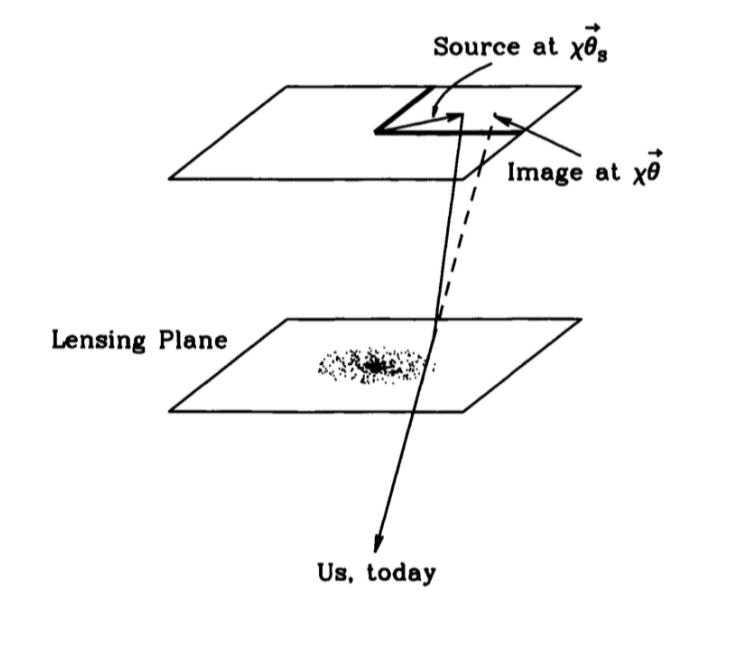
\includegraphics[width=0.5\textwidth]{photon_lensing}
	\caption{Schematic showing the deflection in the path of a photon due to gravitational lensing }
	\label{fig:photon_lensing}
\end{figure}

In the source plane we have defined a set of mutually perpendicular axes denoted by superscript 1 and 2. Therefore, the position of a general point in the source plane will be denoted using two components: ($\chi^{\theta^1}, \chi^{\theta^2}$). Here $\chi$ and $\theta$ are labels. They denote that the point is located at $\chi$ comoving distance away from the observer and makes an angle $\theta$ with the line joining the observer and the center of source plane.


Here $\chi ^{\vec{\theta}_S}$ is the actual position of the photon on the source plane and $\chi^{\vec{\theta}}$ is the apparent position of the source. The spatial position of the photon on the source plane is defined as ($\chi^{\theta^1}, \chi^{\theta^2}, \chi$). Where $\chi$ is the comoving radial distance between the source and observer, and $|\chi^{\vec{\theta}}|$  is the comoving distance of the photon from the origin on the source plane.

The comoving distance \textit{"from the observer to the source"} is given by the relation
\beqa
\chi(a) = \int_{t(a)}^{t_0} \frac{dt^\prime}{a(t^\prime)} = \int_{a}^{1} \frac{da^\prime}{a^\prime H(a^\prime)}
\eeqa

In terms of axis, the $\chi$ vector extends from observer towards source. As photon moves towards the observer, $t^\prime$ increases, $a(t^\prime)$ increases and $|\chi|$ decreases. Therefore, 
\beqa
\frac{d\chi}{dt} = \frac{-1}{a}
\eeqa

We need to rewrite the geodesic equation in terms of the chosen coordinate system. Therefore simplifying the LHS using 
\begin{equation}
\begin{aligned}
\frac{d\chi^{\theta^i}}{d\lambda} &= \frac{dt}{d\lambda} \frac{d\chi}{dt} \frac{d\chi^{\theta^i}}{d\chi} 
\\
& = P^0 \frac{-1}{a} \frac{d\chi^{\theta^i}}{d\chi}
\\
& = \frac{-1}{a} p (1-\Psi) \frac{d \chi^{\theta^i}}{d\chi} \\
& \simeq \frac{-p}{a} \frac{d\chi^{\theta^i}}{d\chi} 
\end{aligned} 
\end{equation}

Similarly, 
\beqa
\frac{d\chi}{d\lambda} = \frac{-p}{a} (1-\Psi)
\label{eq:zero_order_p_a}
\eeqa

Therefore, the LHS of the geodesic equation becomes
\begin{equation}
\begin{aligned}
\frac{d^2\chi^{\theta^i}}{d\lambda^2}  = \frac{p}{a} \frac{d}{d\chi}\left( \frac{p}{a}  \frac{d\chi^{\theta^i}}{d\chi}\right)
\end{aligned}
\end{equation}

On RHS we have,
\begin{equation}
\begin{aligned}
\Gamma^{i}_{\alpha \beta} \frac{dx^{\alpha}}{d\lambda}\frac{dx^{\alpha}}{d\lambda} =  \Gamma^{i}_{\alpha \beta}\frac{p^2}{a^2} (1 - \Psi)^2 \frac{dx^\alpha}{d\chi}\frac{dx^\beta}{d\chi} 
\end{aligned}
\end{equation}

Therefore,
\begin{equation}
\begin{aligned}
\Gamma^{i}_{0\beta} \frac{dt}{d\lambda} \frac{dx^{\beta}}{d\lambda} & = \delta^{i}_\beta (H+\Phi,_{0})  \frac{p^2}{a^2} (1-\Psi)^2 \frac{dt}{d\chi} \frac{dx^\beta}{d\chi} \\
& = \frac{p^2}{a^2} (-a) H \frac{d\chi^{\theta^i}}{d\chi}
\label{eq:rhs1}
\end{aligned}
\end{equation}

In the second equality, using the delta function, we replace $x^\beta$ with the spatial transverse part. Upto first order, we neglect $\Psi$ and substitute $\frac{dt}{d\chi} = -a$.

Now,
\begin{equation}
\begin{aligned}
\Gamma^{i}_{00} (\frac{dt}{d\lambda})^2 & = \frac{\Psi,_{i}}{a^2} (\frac{dt}{d\chi})^2 \\
& = \Psi,_{i} \frac{p^2}{a^2}
& = -\Phi,_{i} \frac{p^2}{a^2}
\label{eq:rhs2}
\end{aligned}
\end{equation}
where the second equality holds since in the late universe there are no anisotropic stresses so $\Phi = - \Psi$. \textcolor{red}{[dodelson]I don't understand this anisotropy part.}


Similarly,
\begin{equation}
\begin{aligned}
\Gamma^{i}_{\alpha \beta} \frac{dx^\alpha}{d\lambda} \frac{dx^{\beta}}{d\lambda} & = (\delta^{i}_{\alpha} \Phi,_{\beta} + \delta ^{i}_{\beta} \Phi, _{\alpha} - \delta_{\alpha \beta}\Phi,_{i} )  \frac{p^2}{a^2} (1-\Psi)^2 \frac{dx^\alpha}{d\chi} \frac{dx^\beta}{d\chi} \\
\end{aligned}
\end{equation}
Here, if $x^\alpha, x^\beta$ are transverse coordinates, then the resulting term after multiplication with $\Phi$ would be very small. Therefore, $\alpha$ and $\beta$ are equal to 3. 
Therefore,
\begin{equation}
\begin{aligned}
\Gamma^{i}_{3 3} \frac{dx^3}{d\lambda} \frac{dx^{3}}{d\lambda} & = (\delta^{i}_{3} \Phi,_{3} + \delta ^{i}_{3} \Phi, _{3} - \delta_{3 3}\Phi,_{i} )  \frac{p^2}{a^2} (1-\Psi)^2 \frac{dx^3}{d\chi} \frac{dx^3}{d\chi} \\
& = - \Phi,_{i} \frac{p^2}{a^2}
\label{eq:rhs3}
\end{aligned}
\end{equation}
The first two terms vanish because $i\neq3$.

Now that we have found out all the terms on RHS. Let's simplify LHS

\begin{equation}
\begin{aligned}
\frac{d^2\chi^{\theta^i}}{d\lambda^2}  &= \frac{p}{a} \frac{d}{d\chi}\left( \frac{p}{a}  \frac{d\chi^{\theta^i}}{d\chi}\right) \\ 
&= \frac{p}{a^2}\frac{dp}{d\chi}\frac{d\chi^{\theta^i}}{d\chi} - \frac{p^2}{a^3}\frac{da}{d\chi} \frac{d\chi^{\theta^i}}{d\chi} + \frac{p^2}{a^2}\frac{d^2 \chi^{\theta^i}}{\chi^2} \\
&= \frac{-2p^2}{a^3} \frac{da}{d\chi} \frac{\chi^{\theta^i}}{d\chi} + \frac{p^2}{a^2} \frac{d^2 \chi^{\theta^i}}{d \chi^2}
\label{eq:lhs}
\end{aligned}
\end{equation}
In the second equality, we just opened the brackets using the chain rule for differentiation. In the third equality, in the first term we used equation \ref{eq:zero_order_p_a} to replace $p$ with $-a \frac{d\chi}{d\lambda}$ upto zeroth order.

Equating equation \ref{eq:lhs}, \ref{eq:rhs1}, \ref{eq:rhs2}, and \ref{eq:rhs3}

\begin{equation}
\begin{aligned}
\frac{-2p^2}{a^3} \frac{da}{d\chi} \frac{\chi^{\theta^i}}{d\chi} + \frac{p^2}{a^2} \frac{d^2 \chi^{\theta^i}}{d \chi^2} &= \frac{p^2}{a^2}\left[ 2\Phi,_i + aH \frac{d\chi^{\theta^i}}{d\chi} \right]
\end{aligned}
\end{equation}

First term on LHS ad second term on RHS cancel and we are left with (inserting $c^2$)
\beqa
\frac{d^2\chi^{\theta^i}}{d\chi^2} = \frac{2 \Phi,_i}{c^2}
\eeqa

\subsection{Reduced deflection angle and lensing potential}
\begin{center}
Ref: Bartelmann, Maturi (arxiv:1612.06535)
\end{center}
After integration, we get
\begin{equation}
\begin{aligned}
\frac{d\chi^{\theta^i}}{d\chi} = \int_{0}^{\chi}\frac{2\Phi,_i}{c^2} d\chi + constant
\end{aligned}
\end{equation}

\beqa
\left. \chi^{\theta^i} \right	|_{limits} = \int_{0}^{\chi} d\chi^{\prime \prime} \int_{0}^{\chi^{\prime \prime}}d\chi^{\prime} \frac{2 \Phi,_i}{c^2}
\label{eq:eqn}
\eeqa

\begin{figure}[h]
    \centering
	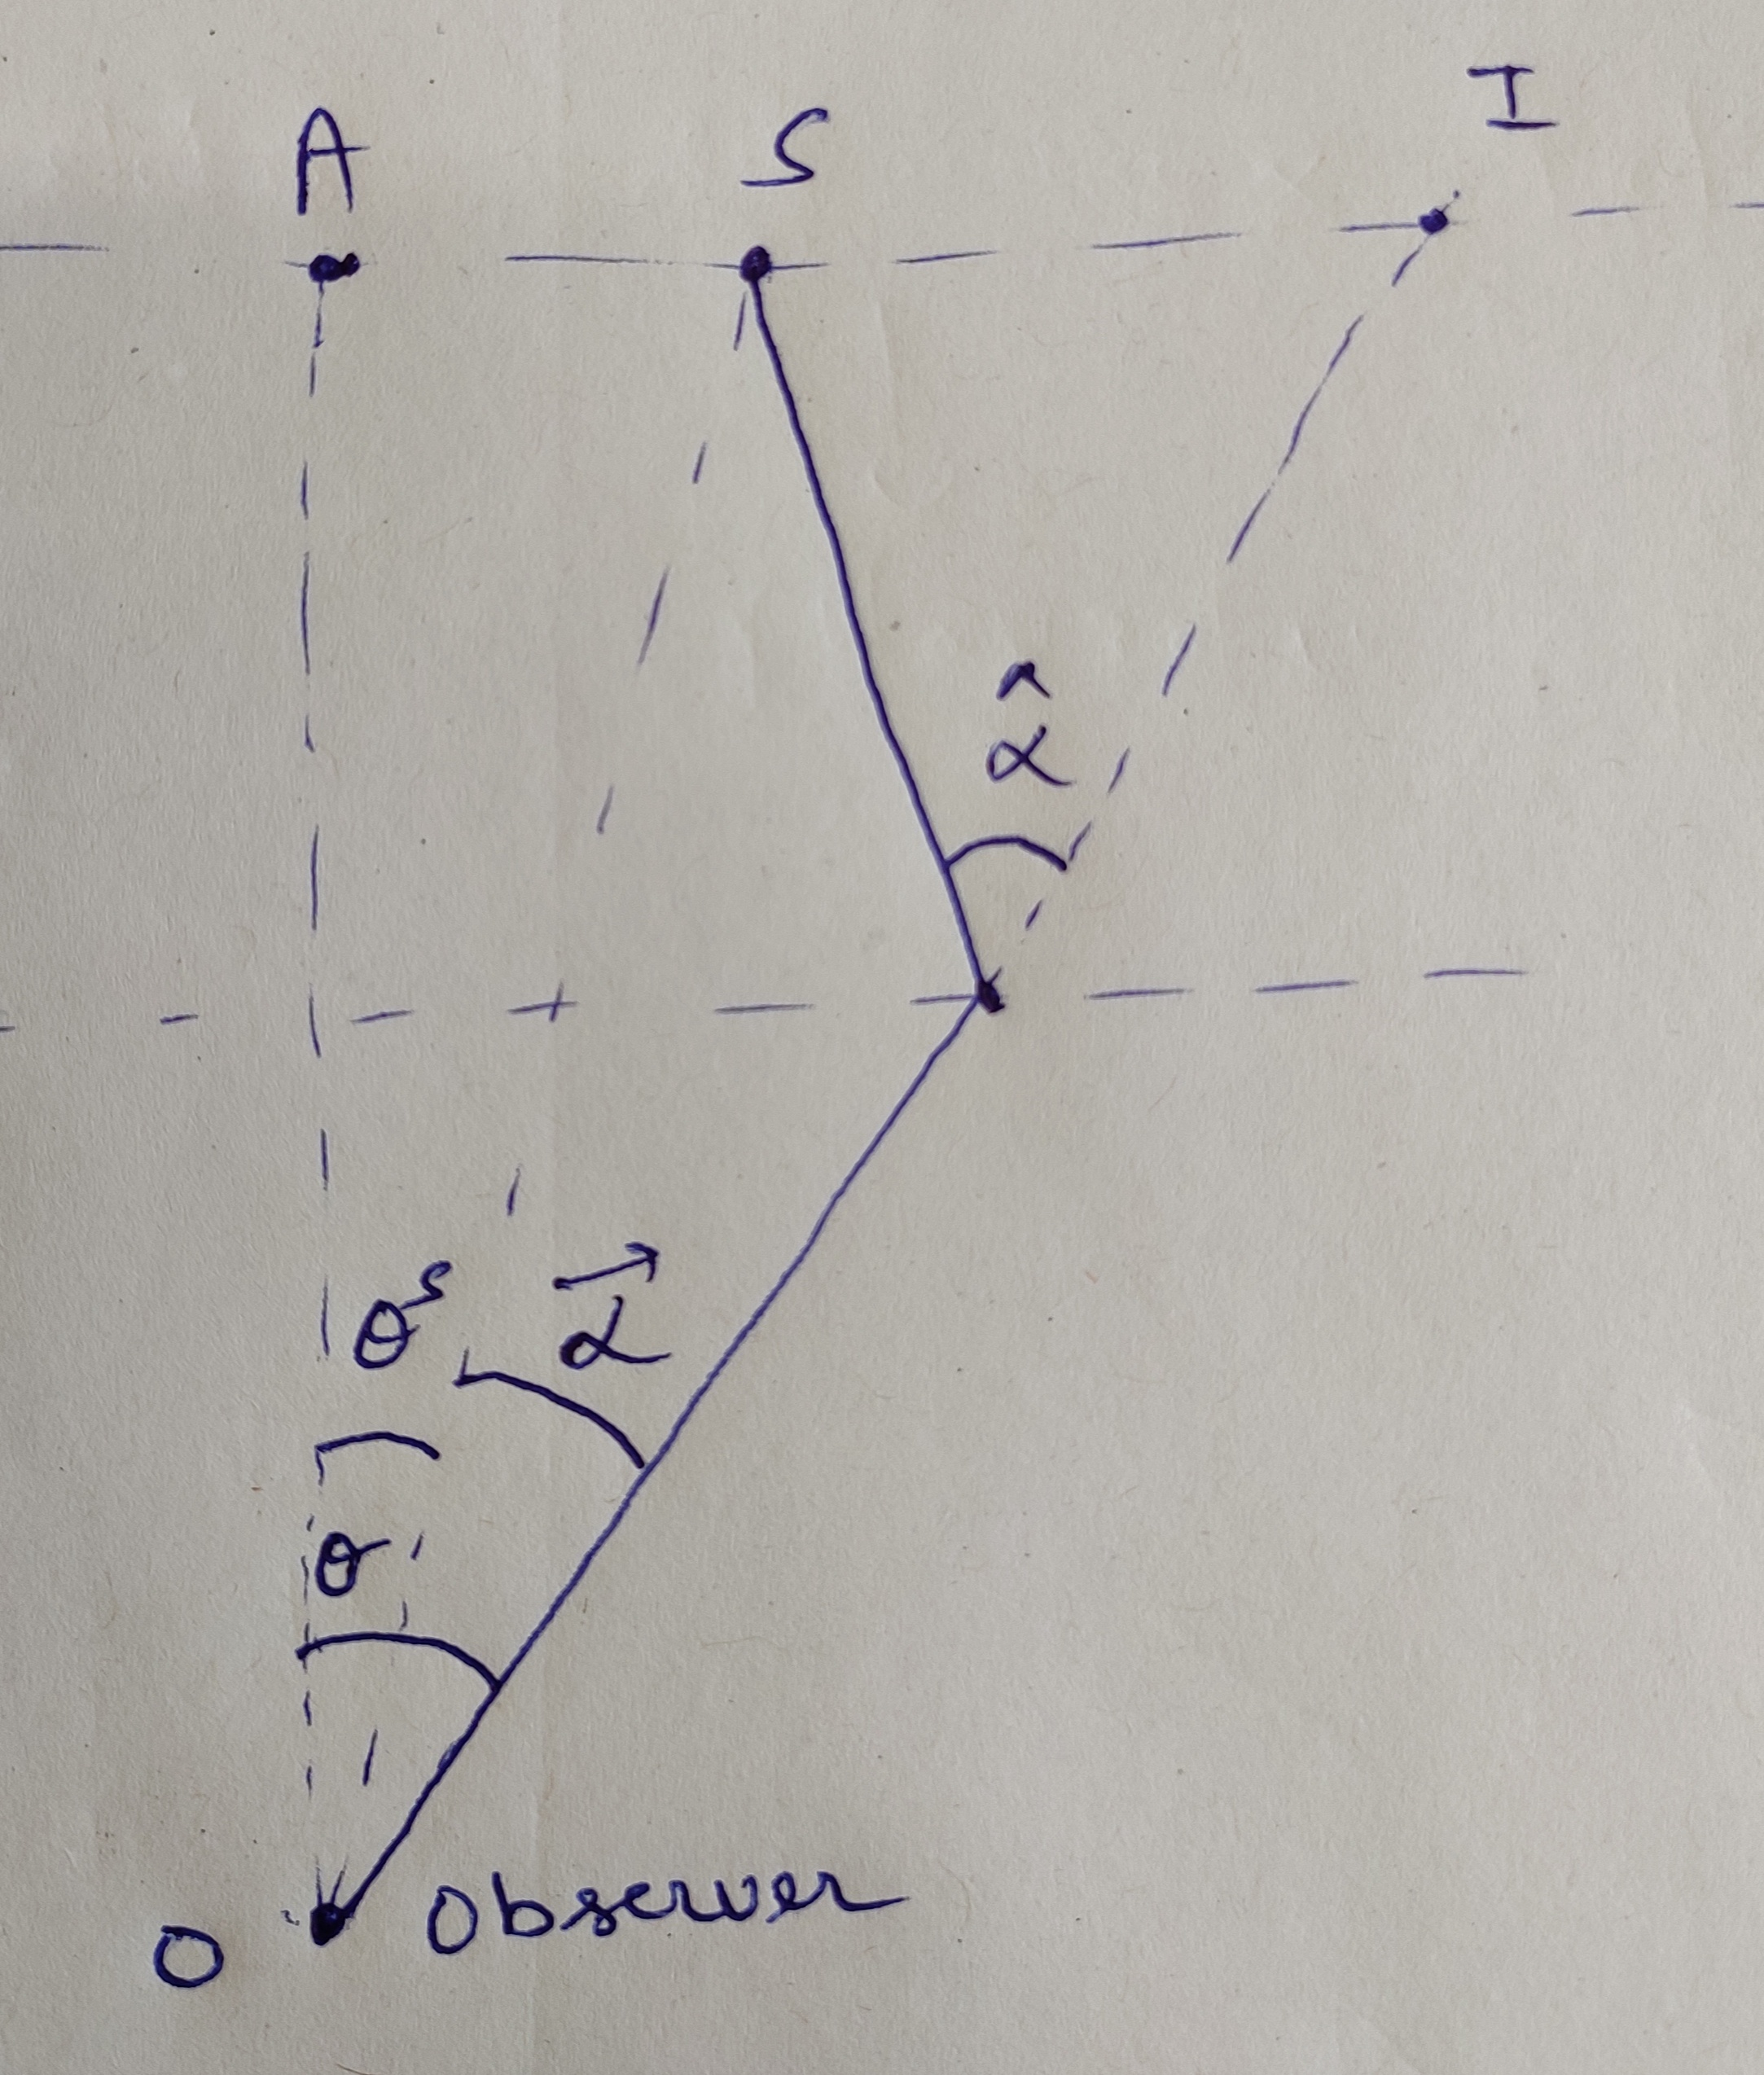
\includegraphics[width=0.25\textwidth, height=4cm]{lensing_schematic}
	\caption{Schematic showing the angular coordinates of source and image}
	\label{fig:lensing_schematic}
\end{figure}


In the schematic, we can see that
\beqa
\frac{\chi^{\theta^i}}{\chi} &= \theta \label{eq:theta}\\ 
\frac{\chi^{\theta_S^i}}{\chi} &= \theta_S \label{eq:theta_s}
\eeqa

This comes from the definition of angular diameter distance
\beqa
\beta = \frac{l}{D_A}
\eeqa

where $\beta$ is the angle subtended by an object of physical size $l$ and at $D_A$ is the angular diameter distance between the source and the observer. 


We have $a\chi^{\theta^i} = l$ and $a\chi = D_A^\chi$. a's cancel and we get equation \ref{eq:theta} and \ref{eq:theta_s}.

Therefore, on dividing \ref{eq:eqn} by $\chi$ on both sides we get
\beqa
\theta_S^i - \theta^i = \frac{1}{\chi}\int_{0}^{\chi} d\chi^{\prime \prime} \int_{0}^{\chi^{\prime \prime}}d\chi^{\prime} \frac{2 \Phi,_i}{c^2} 
\eeqa

writing $\int_{0}^{\chi^{\prime \prime}}d\chi^{\prime} 2 \Phi,_{i} \equiv f(\chi^{\prime \prime})$. Therefore

\begin{equation}
\begin{aligned}
\theta_S^i - \theta^i &= \frac{1}{\chi}\int_{0}^{\chi} d\chi^{\prime \prime} f(\chi^{\prime \prime}) 
\\
& = \frac{1}{\chi} \left( \left[\chi^{\prime \prime} f(\chi^{\prime \prime}) \right]_0^{\chi} - \int_{0}^{\chi} d\chi^{\prime \prime} \frac{df(\chi^{\prime \prime})} {d\chi^{\prime \prime}}\chi^{\prime \prime}  \right)
\\
& = \frac{1}{\chi}\chi f(\chi)- \frac{1}{\chi}\int_{0}^{\chi} d\chi^{\prime \prime} \frac{df(\chi^{\prime \prime})} {d\chi^{\prime \prime}}\chi^{\prime \prime} 
\\
&= \int_{0}^{\chi}d\chi^{\prime} \frac{2 \Phi,_i}{c^2} - \frac{1}{\chi}\int_{0}^{\chi}d\chi^{\prime} \frac{2 \Phi,_i}{c^2}(x(\chi^{\prime})) \chi^{\prime}
\\
&= \int_{0}^{\chi} d\chi^{\prime} \frac{2 \Phi,_i}{c^2}(\vec{x}(\chi^{\prime})) \left(1 - \frac{\chi^{\prime}}{\chi}\right)
\end{aligned}
\end{equation}

where the second equality has been obtained by doing integration by parts. 

Therefore, we finally have the result
\begin{equation}
\begin{aligned}
\theta_S^i - \theta^i = \frac{2}{c^2} \int_{0}^{\chi} d\chi^{\prime} \Phi,_i(\vec{x}(\chi^{\prime})) \left(1 - \frac{\chi^{\prime}}{\chi}\right)
\end{aligned}
\end{equation}

This result refers to the situation when the source is at a fixed distance from the observer. In the case of large scale structure lenses, we would also have to put a redshift distribution function of sources. {\color{red}{refine}}.


In Figure \ref{fig:lensing_schematic}, $S$ is the source, I is the apparent position of the source on the source plane. $\hat{\alpha}$ is the deflection angle. $\vec{\alpha}$ is the reduced deflection angle. 
\beqa
\vec{\theta_S} -\vec{\theta} &= \vec{\alpha} 
\eeqa

Therefore,

\beq
\beqal
\vec{\alpha} &= \vec{\bigtriangledown}_\perp \int_{0}^{\chi} d\chi^{\prime} \frac{2}{c^2}\Phi(\vec{x}(\chi^{\prime})) \left(1 - \frac{\chi^{\prime}}{\chi}\right)
\\
&=  \vec{\bigtriangledown}_\theta  \int_{0}^{\chi} d\chi^{\prime} \frac{2}{c^2}\Phi(\vec{x}(\chi^{\prime})) \left(1 - \frac{\chi^{\prime}}{\chi}\right) \frac{1}{\chi^\prime}
\\
&= \vec{\bigtriangledown}_\theta \psi
\\
\therefore \vec{\theta}_S  &=\vec{\theta}+  \vec{\bigtriangledown}_\theta \psi
\eeqal
\eeq

where, $\psi$ is defined as \textbf{\textit{lensing potential}}. We converted $\vec{\bigtriangledown}_\perp$ to $\vec{\bigtriangledown}_\theta$ because when we measure the position of sources, we measure the  angle subtended by them. Therefore, we want all the derivatives with respect to the angular coordinates.
%
%\beq
%\beqal
%\vec{\theta_S} -\vec{\theta} &= \vec{\alpha} \\
%\chi &\equiv D_S \\
%\chi^\prime &\equiv D_L \\
%\chi - \chi^\prime &\equiv D_{LS} 
%\eeqal
%\eeq
%$D_S = \chi$ is the radial comoving distance between the source and observer. $D_{LS} = \chi - \chi^\prime$ is the comoving distance between the lens and source, and $D_L = \chi^\prime$ is the comoving distance between the observer and the lens.
%
%\beq
%\beqal
%\bigtriangledown_\perp  = D_L^{-1} \bigtriangledown_\theta
%\eeqal
%\eeq
%
%\beq
%\beqal
%\therefore 
%\vec{\alpha} &=  \frac{2}{c^2} \frac{D_{LS}}{D_L D_S} \vec{\bigtriangledown}_\theta \int_0^\chi \Phi(\vec{x(\chi^\prime)}) d\chi^\prime 
%\\
%&= \vec{\bigtriangledown}_\theta \psi
%\eeqal
%\eeq
%
%where $\phi$ is defined as lensing potential

\section{Convergence and shear}
\begin{center}
Ref: Bartelmann, Maturi (arxiv:1612.06535)
\end{center}
\subsection{Convergence}

Using the poisson equation we relate the gravitational potential with the over-density of the region. Similarly, here we want to relate the laplacian of lensing potential with a local quantity. Therefore, we start with

\beq
\beqal
\vec{\bigtriangledown}_\theta \cdot \vec{\alpha} &= \vec{\bigtriangledown}^2_\theta \psi = \frac{2}{c^2}  \int_0^\chi \vec{\bigtriangledown}^2_\perp \left(1 -  \frac{\chi^\prime}{\chi} \right) \chi^\prime \Phi(\vec{x}(\chi^\prime)) d\chi^\prime 
\eeqal
\eeq

The complete Laplacian is 
\beqa
\vec{\bigtriangledown}^2 = \vec{\bigtriangledown}_\perp - \frac{\partial^2}{\partial (\chi^\prime)^2}
\eeqa

If the extent of lensing mass distribution is small compared to the cosmological distances ($D_{LS}$, $D_S$, and $D_L$), then
\beqa
\int \frac{\partial ^2 \Phi}{\partial (\chi^\prime)^2} d\chi^\prime = \left. \frac{\partial \Phi}{\partial \chi^\prime} \right|_{\textrm{end points}} = 0
\eeqa

Therefore, we can replace $\vec{\bigtriangledown}^2_\perp$ with $\vec{\bigtriangledown}^2$ and we get
\beq
\beqal
\vec{\bigtriangledown}_\theta \cdot \vec{\alpha} &= \frac{2}{c^2} \vec{\bigtriangledown}^2  \int_0^\chi \left(1 -  \frac{\chi^\prime}{\chi} \right) \chi^\prime \Phi(\vec{x}(\chi^\prime)) d\chi^\prime 
\eeqal
\eeq


Using the poisson's equation
\beqa
\vec{\bigtriangledown}^2 \Phi  = 4 \pi G \rho
\eeqa

we get

\beq
\beqal
\vec{\bigtriangledown}^2_\theta \psi  &= \frac{ 8 \pi G }{c^2}  \int_0^\chi \left(1 -  \frac{\chi^\prime}{\chi} \right) \chi^\prime  \rho(\vec{x}(\chi^\prime)) a^2 d\chi^\prime 
\\
& = 2\kappa
\eeqal
\eeq

where $\kappa$ is the convergence, defined as
\beq
\beqal
\kappa &= \frac{1}{2} \vec{\bigtriangledown}^2_\theta \psi
\\
&= \frac{4 \pi G }{c^2}   \int_0^\chi \left(1 -  \frac{\chi^\prime}{\chi} \right) \chi^\prime  \rho(\vec{x}(\chi^\prime)) a^2 d\chi^\prime 
\eeqal
\eeq

and $a$ is the scale factor.

This expression shows that convergence is a geometrically weighted line-of-sight integral over mass density $\rho$. $\rho$ is the fluctuation of mass density about its cosmological mean value $\bar{\rho}$ and not the entire mass density.{\color{red} refine} The convergence $\kappa$  thus describes the lensing effects of matter inhomogeneities in an otherwise homogeneous mean universe. Writing $\rho$ as $\rho = \bar{\rho} \delta$, where $\delta$ is dimensionless. In terms of conventional cosmological parameters, the mean matter density is 
\beqa
\bar{\rho} = \frac{3 H_0^2}{8 \pi G} \Omega_{m0} a^{-3}
\eeqa
where $H_0$ is the Hubble constant quantifying the present expansion rate of the universe, and $\Omega_{m0}$ is the dimensionless matter-density parameter. Therefore, we get

\beqa
\kappa (\chi^{\vec{\theta}}) = \frac{3}{2} \frac{H_0^2}{c^2} \Omega_{m0} \int_0^\chi d\chi^\prime \chi^\prime \frac{(\chi - \chi^\prime)}{\chi} \frac{\delta(\vec{\chi}^\prime)}{a} \label{eq:eff_convergence}
\eeqa

for the convergence $\kappa$ of an extended lens. It is called \textit{effective convergence} because it corresponds to the convergence of a thin lens whose effects are equivalent to those caused by the actual extended matter distribution. Again, this expression is true for a fixed source. For extended large scale structure, we would have to put the source redshift distribution function in the expression.

\beqa
\kappa (\chi^{\vec{\theta}})= \int_0^{\chi} d\chi^\prime W(\chi^\prime,\chi) \delta (\vec{\chi}^\prime))
\eeqa


%\subsection{Statiatics of density field}
%\beqa
%\langle \delta(\vec{x}) = 0 \rangle
%\eeqa
%
%\textit{correlation function}
%\beqa
%\xi(\vec{x}, \vec{y}) \equiv \langle \delta(\vec{x}) \delta(\vec{y}) \rangle
%\eeqa
%
%where brackets denote the average over all space. Universe is homogeneous, therefore the correlation function should depend only on the difference between $\vec{x}$ and $\vec{y}$. 
%\beqa
%\xi(\vec{x}, \vec{y}) = \xi (\vec{x} - \vec{y})
%\eeqa
%
%Isotropy of universe requires that the correlation should depend only on the magnitude of distance $\vec{x} - \vec{y}$ and not on its orientation. 
%\beqa
%\xi(\vec{x} - \vec{y})= \xi(|\vec{x} - \vec{y}|)
%\eeqa
%
%\begin{figure}[h]
%	\centering
%	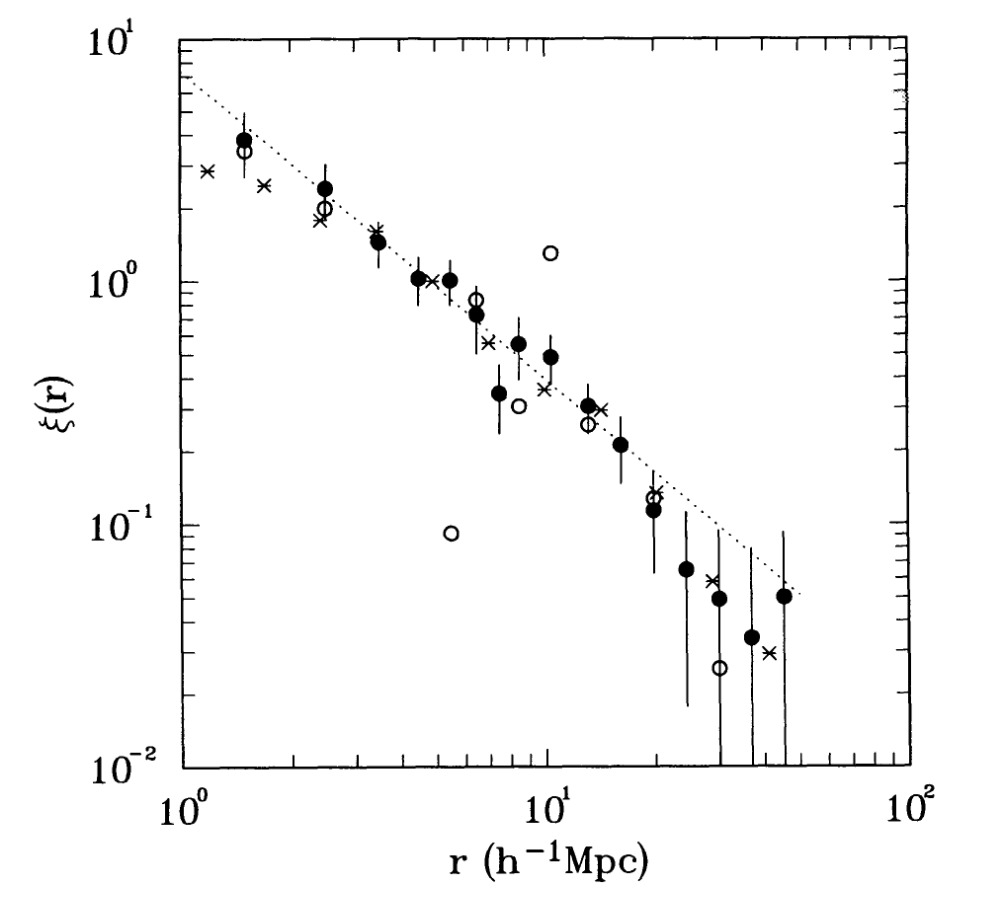
\includegraphics[width=0.5\textwidth]{correlation_qdot}
%	\caption{The correlation fuction as measured in the QDOT survey (\cite{correlation_qdot}). The different symbols are different ways of estimating the correlation function; the all agree quantitatively that galaxies are clumped on small scales, where $\xi > 1$, but are distributed relatively smoothly on larger scales}
%	\label{correlation_qdot}
%\end{figure}
%
%Fig. \ref{correlation_qdot} shows the correlation function of galaxies mapped in the QDOT survey. A value greater than unity means that two nearby regions are correlated and therefore likely to have similar values of $\delta$. From the figure we see that this holds for distances smaller than $\sim 10$ Mpc. On larger scales, correlation is much weaker. That is, at a distance of $20$ Mpc, you should not expect to find any over densities; or, at least, not any more than you would in a random place. This qualitative feature of the correlation function tells us that the universe is clumpy on small scales but smooth on large scales. 
%
%We have 
%\beqa
%\delta(\vec{x}) = \int \frac{d^3\kappa}{(2\pi)^3} \tilde{\delta}(\vec{\kappa}) e^{i\vec{\kappa}.  \vec{x}}
%\eeqa
%and 
%\beqa
%\tilde{\delta}(\vec{\kappa}) = \int d^3x \delta(\vec{\x}) e^{-i\vec{\kappa}.  \vec{x}}
%\eeqa
%
%mean of $\tilde{\delta}(\vec{\kappa})$ vanishes, but the product of two $\tilde{\delta}$s encode a lot of information about the structure of the universe.
%
%Consider
%\beqa
%\langle \tilde{\delta}(\vec{\kappa})\tilde{\delta}(\vec{\kappa}^\prime) \rangle = \int d^3 x e^{-i \vec{\kappa}. \vec{x}} \int d^y e^{-\vec{\kappa}^\prime . \vec{y}} \xi(\vec{x} - \vec{y})
%\eeqa
%
%
%where $\langle  \delta(\vec{x}) \delta(\vec{y})) = \xi (\vec{x} - \vec{y})\rangle$
%
%using $\vec{x}_- = \vec{x} - \vec{y}$
%
%\beq
%\beqal
%\langle\tilde{\delta}(\vec{\kappa})\tilde{\delta}(\vec{\kappa}^\prime)  \rangle = \int d^3x e^{-i(\vec{\kappa} - \vec{\kappa}^\prime)\cdot \vec{x}_-} \xi(\vec{x}_-) 
%\\
%&= (2\pi)^3 \delta_D (\vec{\kappa} - \vec{\kappa}^\prime) \int d^3x_- e^{i\vec{\kappa}^\prime \cdot x_-} \xi(\vec{x}_-)
%\\
%&= (2\pi)^3 \delta_D(\vec{\kappa}+ \vec{\kappa}^\prime)P(k)
%\eeqal
%\eeq
%
%$P(\kappa)$ is the power spectrum. Note that, since $\xi$ depends only on the magnitude of $\vec{x}_-$, the power spectrum depends only on the magnitude of its argument of $P = P(|\vec{\kappa}|)$.
%
%{\color{red} Dirac delta enforces the fact that the fluctuations in the fourier modes are correlated with one another only if the two modes have eqlau and opposite wave vectors.}
%
%\beqa
%insert BOSS figure
%\eeqa
%If we plot $P(k)$ we the power falls as $k$ increases. It looks like there is more power on large scales than on small scales which means that the universe is smooth on small scales and clumpy on large scales. 
%
%To understand this, let's look at the variance of density  fluctuations
%\beqa
%\sigma^2 \equiv \langle \delta^2(\vec{x}) \rangle
%\eeqa
%
%Fourier transform gives
%\beq
%\sigma^2 = \int \frac{d^3k}{(2\pi)^3} \int \frac{d^3k}{(2\pi)^3} e^{i\vec{x} \cdot (\vec{\kappa} + \vec{\kappa}^\prime)} \langle \tilde{\delta}(\vec{\kappa}) \tilde{\delta}(\vec{\kappa}^\prime) \rangle
%\eeq
%
%which simplifies using Equation .. to 
%\beq
%\beqal
%\sigma^2 = \int \frac{d^3\kappa}{(2\pi)^3} P(\kappa)
%\\
%&= \int_0^{\infty} \frac{d\kappa}{\kappa} \frac{\kappa^3 P(\kappa)}{2\pi^2}
%\eeqal
%\eeq


\subsection{Statitstics of convergence field}
\beqa
\langle \tilde{\kappa}(\vec{l}) \tilde{\kappa}(\vec{l}^\prime)\rangle = (2\pi)^2 \delta_D^2 (\vec{l} + \vec{l}^\prime) C_l^{\kappa \kappa}
\eeqa

Power spectrum depends only on the magnitude of the wave vector $\vec{l}$, not its direction. Analogous to the 3D case, each angular scale $l$ has fluctuation with variance $l^2 C_l^{\kappa \kappa} / 2 \pi$,. The variance of the fluctuations of the convergence field will be the logarithmic integral over all $l$ of $l^2 C_l^{\kappa \kappa}/2\pi$.

\subsection{Errors on the convergence power spectrum}

\subsection{Shear}
Using the relation
\beqa
\vec{\theta}_S = \vec{\theta} - \vec{\bigtriangledown}_\theta\psi 
\eeqa

we get the Jacobian matrix as 
4%% %
%\subsection{sdfgfdsadfgfds}
%The presence of index $i$ in this expression shows that in general different components of the position vector change differently. ($\theta^i$ denotes the angle made by the $i^{th}$ component of the position vector.) This results in the distortion of the shape of bodies. 
%
%Since $\Phi$ depends on $\chi^{\vec{{\theta}}}$, we can define the rate of change of angles in different directions.

\beq
\beqal
A_{ij}(\chi_S, \theta) &\equiv \frac{\partial\theta_S^i}{\partial\theta^j} 
\\
&= \delta_{ij} - \psi,_{ij}
%\\
%&= \frac{2}{c^2}  \int_0^\chi \vec{\bigtriangledown}^2_\perp \left(1 -  \frac{\chi^\prime}{\chi} \right) \chi^\prime \Phi(\vec{x}(\chi^\prime)) d\chi^\prime 
%\\
%&= \delta_{ij} - \frac{2}{c^2} \int d\chi^\prime g(\chi^\prime)  \Phi,_{ij}(\vec{x}(\chi^\prime)) 
\eeqal
\eeq

where subscripts in $\psi_{ij}$ denote derivatives w.r.t. components of $\vec{\theta}$.

We split the jacobi matrix into isotropic and anisotropic (trace-free) part

\beq
\beqal
tr(A) = 2 - \vec{\bigtriangledown}^2 \psi = 2(1-\kappa)
\eeqal
\eeq

Where, $tr(\psi,_{ij})$ gives the diagonal elements which is equal to $\vec{\bigtriangledown}^2 \psi$

Using this we obtain the shear matrix by removing the isotropic part from $A$
\beq
\beqal
\Gamma &=  \left( A - \frac{1}{2} [tr (A)] I \right)
\\
&= \left( [\delta_{ij} - \psi,_{ij}]_\textrm{matrix} - (1-k)I \right)
\\
&= -[\psi_{ij}]_\textrm{matrix} - (1-k)I
\\
&= -\left([\psi_{ij}]_\textrm{matrix} + (1-k)I \right)
\eeqal
\eeq

We have $k = \frac{1}{2} (\psi_{11} + \psi_{22})$, using this we finally get

It's components are
\beq
\beqal
\Gamma_{11} &= - \gamma_1 = -\frac{1}{2} (\psi_{11} - \psi_{22})
\\
\Gamma_{22} &= \gamma_1 
\\
\Gamma_{12} &= \Gamma_{21} = - \gamma_2 = - \psi_{12}
\eeqal
\eeq

Therefore,
\beq
\beqal
A &= 
\begin{pmatrix}
1 - \kappa - \gamma_1 & -\gamma_{12} 
\\
-\gamma_{21} & 1 - \kappa + \gamma_1
\end{pmatrix} 
\\
&= (1-\kappa) 
\begin{pmatrix}
1 & 0 \\
0 & 1 \\
\end{pmatrix}
+
\begin{pmatrix}
- \gamma_1 & -\gamma_{12} \\
-\gamma_{21} & \gamma_1 \\
\end{pmatrix}
\eeqal
\eeq

Convergence causes an isotropic magnification of angular size in the neighborhood of $\vec{\theta}$ while shear produces anisotropy.

For a small circular source, its lensed image is an ellipse, with major and minor axes
\beqa
a = (1 - \kappa - \gamma_1)^{-1} \textrm{and} \; b = (1 - \kappa + \gamma_1)^{-1}
\eeqa

\section{Cosmological weak gravitational lensing }
\begin{center}
Ref: Bartelmann, Maturi (arxiv:1612.06535)
\end{center}
\subsection{Limber's approximation}
If the quantity $x(\vec{\theta})$ defined in two dimensions is a projection
\beqa
x(\vec{\theta}) = \int_0^\chi d\chi^\prime w(\chi^\prime) y(\vec{x}(\chi^\prime))
\eeqa

of a quantity $y(\vec{r})$ defined in three dimensions with a weight function $w(\chi^\prime)$, then the angular power spectrum of $x$ is given by 
\beqa
C_x(l) = \int_0^\chi d\chi^\prime \frac{w^2(\chi^\prime)}{(\chi^\prime)^2} P_y \left( \frac{l}{\chi^\prime} \right)
\eeqa

where $P_y(k)$ is the power spectrum of $y$, taken at the three dimensional wave number $k= l/\chi^\prime$. The condition of applicability of the approximation is that $y$ must vary on length scales much smaller than the typical length scale of the weight.

%\subsection{Convergence power spectrum}
%
%Using Equation \ref{eq:eff_convergence}, we write the two point function of the convergence field
%\begin{equation}
%\langle \kappa(\chi^{\vec{\theta}}) \kappa(\chi^{\vec{\theta'}})\rangle = \frac{9 H_0^2 \Omega_{m0}^2}{4 c^4} \int_0^{\chi_S} d\chi \int_0^{\chi_S} d\chi'  \left(\frac{\chi_S - \chi}{\chi_S}\right) \left(\frac{\chi_S - \chi'}{\chi_S}\right) \chi \chi' \frac{1}{a^2} \langle\delta(\vec{\chi}) \delta(\vec{\chi}') \rangle 
%\end{equation}
%
%%Using equation \ref{eq:correlation_function}, we rewrite this result as 
%%\begin{equation}
%%\langle \kappa(\chi) \kappa(\chi')\rangle = \frac{9 H_0^2 \Omega_{m0}^2}{4 c^4} \int_0^{\chi_S} d\chi \int_0^{\chi_S} d\chi'  \left(\frac{\chi_S - \chi}{\chi_S}\right) \left(\frac{\chi_S - \chi'}{\chi_S}\right) \chi \chi' \frac{1}{a^2} \langle\delta(\chi) \delta(\chi') \rangle 
%%\end{equation}
%
%Here,
%
%\begin{eqnarray}
%\langle\delta(\vec{\chi}) \delta(\vec{\chi}') \rangle  
%&=& \langle \int \frac{d^3k}{(2\pi)^3} \int \frac{d^3k'}{(2\pi)^3} e^{ik\chi} e^{ik'\chi'} \delta(\vec{k}) \delta(\vec{k}') \rangle 
%\\
% &=&  \int \frac{d^3k}{(2\pi)^3} \int_0^{k} \frac{d^3k'}{(2\pi)^3} e^{ik\chi} e^{ik'\chi'} \langle\delta(\vec{k}) \delta(\vec{k}') \rangle 
% \\
% &=& \int \frac{d^3k}{(2\pi)^3} \int \frac{d^3k'}{(2\pi)^3} e^{ik\chi} e^{i(k' + k - k)\chi'} \langle\delta(\vec{k}) \delta(\vec{k}') \rangle 
% \\
% &= & \int \frac{d^3k}{(2\pi)^3} \int  \frac{d^3k'}{(2\pi)^3} e^{ik(\chi - \chi')} e^{i(k' + k )\chi'} \langle\delta(\vec{k}) \delta(\vec{k}') \rangle 
%\end{eqnarray}
%Let's write $\langle \delta(\vec{k}) \delta(\vec{k}') \rangle \equiv \xi(\vec{k}_d)$, where, $ \vec{k}_d \equiv \vec{k}+\vec{k}' $ 
%Therefore,
%\begin{eqnarray}
%\langle\delta(\vec{\chi}) \delta(\vec{\chi}') \rangle = \int \frac{d^3\vec{k}}{(2\pi)^3}  e^{i\vec{k}(\chi - \chi')} \int \frac{d^3\vec{k}_d}{(2\pi)^3} e^{i(\vec{k}_d )\chi'} \xi(\vec{k}_d)
%\end{eqnarray}
%Writing $ \int \frac{d\vec{k}_d}{(2\pi)^3} e^{i(\vec{k}_d )\chi'} \xi(\vec{k}_d) \equiv P(\vec{\chi}') $, where we $ P(\vec{\chi}') $ is the power spectrum.
%Thus,
%\begin{eqnarray}
%\langle\delta(\vec{\chi}) \delta(\vec{\chi}') \rangle =\delta(\vec{\chi} - \vec{\chi}') P(\vec{\chi}')
%\end{eqnarray}
%
%Using this result, we further get
%\begin{eqnarray}
%\langle \kappa(\vec{\chi}) \kappa(\vec{\chi}')\rangle 
%&=& \frac{9 H_0^2 \Omega_{m0}^2}{4 c^4} \int_0^{\chi_S} d\chi \int_0^{\chi_S} d\chi'  \left(\frac{\chi_S - \chi}{\chi_S}\right) \left(\frac{\chi_S - \chi'}{\chi_S}\right) \chi \chi' \frac{1}{a^2} \delta(\vec{\chi} - \vec{\chi}') P(\vec{\chi}')
%\nonumber \\ 
%&=&\frac{9 H_0^2 \Omega_{m0}^2}{4 c^4} \int_0^{\chi_S} d\chi   \left(\frac{\chi_S - \chi}{\chi_S}\right)^2  \chi^2 \frac{1}{a^2} P(\vec{\chi})
%\end{eqnarray}
%
%From equation \ref{eq:eff_convergence}, we have 
%\beqa
%w(\chi^\prime) = \frac{3 H_0^2}{2c^2} \Omega_{m0} \frac{\chi^\prime (\chi - \chi^\prime)}{a \chi}
%\eeqa
%
%Therefore
%\beqa
%C_\kappa(l) = \left(\frac{3 H_0^2}{2c^2} \Omega_{m0} \right)^2 \int_0^{\chi_S} d\chi \left[ \frac{(\chi_S - \chi)}{\chi_S} \frac{1}{a} \right]^2 P_\delta\left( \frac{l}{\chi}\right)
%\eeqa

\subsection{Convergence power spectrum }

Using Equation \ref{eq:eff_convergence}, we write the two point function of the convergence field
\begin{equation}
\langle \kappa(\chi^{\vec{\theta}}) \kappa^*(\chi^{\vec{\theta'}})\rangle = \frac{9 H_0^2 \Omega_{m0}^2}{4 c^4} \int_0^{\chi_S} d\chi \int_0^{\chi_S} d\chi'  \left(\frac{\chi_S - \chi}{\chi_S}\right) \left(\frac{\chi_S - \chi'}{\chi_S}\right) \chi \chi' \frac{1}{a^2} \langle\delta(\vec{\chi}) \delta^*(\vec{\chi}') \rangle 
\end{equation}

%Using equation \ref{eq:correlation_function}, we rewrite this result as 
%\begin{equation}
%\langle \kappa(\chi) \kappa(\chi')\rangle = \frac{9 H_0^2 \Omega_{m0}^2}{4 c^4} \int_0^{\chi_S} d\chi \int_0^{\chi_S} d\chi'  \left(\frac{\chi_S - \chi}{\chi_S}\right) \left(\frac{\chi_S - \chi'}{\chi_S}\right) \chi \chi' \frac{1}{a^2} \langle\delta(\chi) \delta(\chi') \rangle 
%\end{equation}

Here,

\begin{eqnarray}
\langle\delta(\vec{\chi}) \delta^*(\vec{\chi}') \rangle  
&=& \langle \int \frac{d^3k}{(2\pi)^3} \int \frac{d^3k'}{(2\pi)^3} e^{ik\chi} e^{-ik'\chi'} \delta(\vec{k}) \delta^*(\vec{k}') \rangle 
\\
&=&  \int \frac{d^3k}{(2\pi)^3} \int_0^{k} \frac{d^3k'}{(2\pi)^3} e^{ik\chi} e^{-ik'\chi'} \langle\delta(\vec{k}) \delta^*(\vec{k}') \rangle 
\\
&=& \int \frac{d^3k}{(2\pi)^3} \int \frac{d^3k'}{(2\pi)^3} e^{ik\chi} e^{-i(k' + k - k)\chi'} \langle\delta(\vec{k}) \delta^*(\vec{k}') \rangle 
\\
&= & \int \frac{d^3k}{(2\pi)^3} \int  \frac{d^3k'}{(2\pi)^3} e^{ik(\chi - \chi')} e^{i(k - k' )\chi'} \langle\delta(\vec{k}) \delta^*(\vec{k}') \rangle 
\\
&= & \int \frac{d^3k}{(2\pi)^3} \int  \frac{d^3k'}{(2\pi)^3} e^{ik(\chi - \chi')} e^{-i(k' - k )\chi'} \langle\delta(\vec{k}) \delta^*(\vec{k}') \rangle 
\end{eqnarray}

Let's write $\langle \delta(\vec{k}) \delta^*(\vec{k}') \rangle \equiv \xi(\vec{k}_d)$, where, $ \vec{k}_d \equiv \vec{k}-\vec{k}' $ 
Therefore,
\begin{eqnarray}
\langle\delta(\vec{\chi}) \delta^*(\vec{\chi}') \rangle = \int \frac{d^3\vec{k}}{(2\pi)^3}  e^{i\vec{k}(\chi - \chi')} \int \frac{d^3\vec{k}_d}{(2\pi)^3} e^{i(\vec{k}_d )\chi'} \xi(\vec{k}_d)
\end{eqnarray}
Writing $ \int \frac{d\vec{k}_d}{(2\pi)^3} e^{i(\vec{k}_d )\chi'} \xi(\vec{k}_d) \equiv P(\vec{\chi}') $, where we $ P(\vec{\chi}') $ is the power spectrum.
Thus,
\begin{eqnarray}
\langle\delta(\vec{\chi}) \delta^*(\vec{\chi}') \rangle =\delta(\vec{\chi} - \vec{\chi}') P(\vec{\chi}')
\end{eqnarray}

Using this result, we further get
\begin{eqnarray}
\langle \kappa(\vec{\chi}^\theta) \kappa^*(\vec{\chi}^{\theta'})\rangle 
&=& \frac{9 H_0^2 \Omega_{m0}^2}{4 c^4} \int_0^{\chi_S} d\chi \int_0^{\chi_S} d\chi'  \left(\frac{\chi_S - \chi}{\chi_S}\right) \left(\frac{\chi_S - \chi'}{\chi_S}\right) \chi \chi' \nonumber
\\ 
&&  \frac{1}{a^2} \delta(\vec{\chi} - \vec{\chi}') \int \frac{d\vec{k}_d}{(2\pi)^3} e^{i(\vec{k}_d )\chi'} \xi(\vec{k}_d))  
\\
&=& \frac{9 H_0^2 \Omega_{m0}^2}{4 c^4} \int_0^{\chi_S} d\chi \int_0^{\chi_S} d\chi'  \left(\frac{\chi_S - \chi}{\chi_S}\right) \left(\frac{\chi_S - \chi'}{\chi_S}\right) \chi \chi'  \nonumber
\\
&& \frac{1}{a^2} \delta(\vec{\chi} - \vec{\chi}') P(\vec{\chi}')
\\ 
&=&\frac{9 H_0^2 \Omega_{m0}^2}{4 c^4} \int_0^{\chi_S} d\chi   \left(\frac{\chi_S - \chi}{\chi_S}\right)^2  \chi^2 \frac{1}{a^2} P(\vec{\chi})
\end{eqnarray}

Instead of finding out the convergence in real space, let's find write down the convergence and its correlation function in Fourier space. Let's begin with convergence,

\begin{eqnarray}
\kappa (\chi^{\vec{\theta}}) 
&=& \frac{3}{2} \frac{H_0^2}{c^2} \Omega_{m0} \int_0^{\chi_S} d\chi \chi \frac{(\chi_S - \chi)}{\chi_S} \frac{\delta(\vec{\chi})}{a} 
\end{eqnarray}
We rewrite the equation as 
\begin{eqnarray}
\kappa (\vec{\theta})  &=&  \int_0^{\chi_S} d\chi W(\chi_S, \chi) \delta(\vec{\theta} \chi, \chi)
\end{eqnarray}

In Fourier space,
\begin{eqnarray}
\kappa(\vec{l}) 
&=& \int d^2\theta e^{-i\vec{l}\cdot\vec{\theta}}\int_0^{\chi_S}d\chi W(\chi, \chi_S) \int \frac{d^3 \vec{k}}{(2\pi)^3} e^{i\vec{k}\cdot\vec{\chi}} \delta(\vec{k})
\\
&=& \int d^2\theta e^{-i\vec{l}\cdot\vec{\theta}}\int_0^{\chi_S}d\chi W(\chi, \chi_S) \int \frac{d^2 \vec{k}_\perp}{(2\pi)^2}\int \frac{d\vec{k_\parallel}}{2\pi} e^{i\vec{k}\cdot\vec{\chi}} \delta(\vec{k}_\perp, k_\parallel)
\\
&=& \int_0^{\chi_S}d\chi W(\chi, \chi_S) \int \frac{d^2 \vec{k}_\perp}{(2\pi)^2}\int \frac{d\vec{k_\parallel}}{2\pi} \int d^2\theta e^{-i(\vec{l} - \vec{k}_\perp \chi )\cdot\vec{\theta}} e^{i\vec{k}_\parallel \cdot \vec{\chi}} \delta(\vec{k}_\perp, k_\parallel)
\end{eqnarray}

The $ \theta $ integral gives a delta function
\begin{eqnarray}
\kappa(\vec{l}) 
&=& \int_0^{\chi_S}d\chi W(\chi, \chi_S) \int \frac{d^2 \vec{k}_\perp}{(2\pi)^2}\int \frac{d\vec{k_\parallel}}{2\pi} (2\pi)^2 \delta(\vec{l} - \vec{k}_\perp \chi) e^{i\vec{k}_\parallel \cdot \vec{\chi}} \delta(\vec{k}_\perp, k_\parallel)
\\
&=& \int_0^{\chi_S}d\chi W(\chi, \chi_S) \int \frac{d^2 \vec{l}}{(\chi)^2}\int \frac{d\vec{k_\parallel}}{2\pi}  \delta(\vec{l} - \vec{k}_\perp \chi) e^{i\vec{k}_\parallel \cdot \vec{\chi}} \delta(\vec{k}_\perp, k_\parallel)
\\
&=& \int_0^{\chi_S}d\chi \frac{W(\chi, \chi_S)}{\chi^2} \int d^2 \vec{l}\int \frac{d\vec{k_\parallel}}{2\pi}  \delta(\vec{l} - \vec{k}_\perp \chi) e^{i\vec{k}_\parallel \cdot \vec{\chi}} \delta(\vec{k}_\perp, k_\parallel)
\\
&=& \int_0^{\chi_S}d\chi \frac{W(\chi, \chi_S)}{\chi^2} \int \frac{d\vec{k_\parallel}}{2\pi}   e^{i\vec{k}_\parallel \cdot \vec{\chi}} \delta(\frac{\vec{l}}{\chi}, k_\parallel)
\end{eqnarray}

Now, we proceed to find the correlation function
\begin{eqnarray}
\langle \kappa(l) \kappa(l') \rangle 
&=& \langle \int_0^{\chi_S} d\chi \frac{W(\chi, \chi_S)}{\chi^2} \int \frac{d\vec{k_\parallel}}{2\pi}   e^{i\vec{k}_\parallel \cdot \vec{\chi}} \delta(\frac{\vec{l}}{\chi}, k_\parallel) \times \nonumber \\
&& \int_0^{\chi_S} d\chi' \frac{W(\chi', \chi_S)}{\chi'^2} \int \frac{d\vec{k_\parallel}}{2\pi}   e^{i\vec{k}'_\parallel \cdot \vec{\chi'}} \delta(\frac{\vec{l}'}{\chi'}, k_\parallel) \rangle
\\
&=&  \int_0^{\chi_S} d\chi \frac{W(\chi, \chi_S)}{\chi^2} \int_0^{\chi_S} d\chi' \frac{W(\chi', \chi_S)}{\chi'^2} \int \frac{d\vec{k_\parallel}}{2\pi}   e^{i\vec{k}_\parallel \cdot \vec{\chi}}
\\  
&&  \int \frac{d\vec{k_\parallel}}{2\pi}e^{i\vec{k}'_\parallel \cdot \vec{\chi'}}  \langle\delta(\frac{\vec{l}}{\chi}, k_\parallel)\delta(\frac{\vec{l}'}{\chi'}, k'_\parallel) \rangle
\end{eqnarray}

We rewrite the term inside the angular brackets using the Equation \ref{eq:correlation_function}. 

\begin{eqnarray}
\langle \kappa(l) \kappa(l') \rangle 
&=&
\int_0^{\chi_S} d\chi \frac{W(\chi, \chi_S)}{\chi^2} \int_0^{\chi_S} d\chi' \frac{W(\chi', \chi_S)}{\chi'^2} \int \frac{d\vec{k_\parallel}}{2\pi}   e^{i\vec{k}_\parallel \cdot \vec{\chi}}
\\  
&&  \int \frac{d\vec{k_\parallel}}{2\pi}e^{i\vec{k}'_\parallel \cdot \vec{\chi'}}  (2\pi)^2 \delta(\frac{\vec{l}}{\chi} + \frac{\vec{l}'}{\chi'}) P(\frac{\vec{l}'}{\chi'}, k'_z) (2\pi) \delta(k_\parallel + k'_\parallel)
\\
&=&
\int_0^{\chi_S} d\chi \frac{W(\chi, \chi_S)}{\chi^2} \int_0^{\chi_S} d\chi' \frac{W(\chi', \chi_S)}{\chi'^2}   
\\  
&& \int \frac{d\vec{k_\parallel}}{2\pi} e^{i\vec{k}_\parallel \cdot (\vec{\chi} - \vec{\chi}')}   (2\pi)^2 \delta(\frac{\vec{l}}{\chi} + \frac{\vec{l}'}{\chi'}) P(\frac{\vec{l}'}{\chi'}, k_z) 
\end{eqnarray}

Let's take a break and connect this expression with the angular power spectrum. The relation between the two is
\begin{eqnarray}
\langle  \kappa (\vec{l}) \kappa(\vec{l}')\rangle = (2\pi)^2 \delta(\vec{l}+\vec{l}') C_l^{kk}
\end{eqnarray}
Therefore,
\begin{eqnarray}
C_l^{kk} = \int \frac{d^2 l'}{(2\pi)^2} \langle  \kappa (\vec{l}) \kappa(\vec{l}')\rangle
\end{eqnarray}

Substituting the expression of the term in angular brackets, we get
\begin{eqnarray}
C_l^{kk} &=& \int \frac{d^2 l'}{(2\pi)^2} \int_0^{\chi_S} d\chi \frac{W(\chi, \chi_S)}{\chi^2} \int_0^{\chi_S} d\chi' \frac{W(\chi', \chi_S)}{\chi'^2} 
\\  
&&  \int \frac{d\vec{k_\parallel}}{2\pi} e^{i\vec{k}_\parallel \cdot (\vec{\chi} - \vec{\chi}')}  (2\pi)^2 \delta(\frac{\vec{l}}{\chi} + \frac{\vec{l}'}{\chi'}) P(\frac{\vec{l}'}{\chi'}, k_z) 
\\
&=& \int_0^{\chi_S} d\chi \frac{W(\chi, \chi_S)}{\chi^2} \int_0^{\chi_S} d\chi' \frac{W(\chi', \chi_S)}{\chi'^2} 
\\  
&&  \int \frac{d\vec{k_\parallel}}{2\pi} e^{i\vec{k}_\parallel \cdot (\vec{\chi} - \vec{\chi}')}  \int d^2 l'\delta(\frac{\vec{l}}{\chi} + \frac{\vec{l}'}{\chi'}) P(\frac{\vec{l}'}{\chi'}, k_z) 
\\
&=& \int_0^{\chi_S} d\chi \frac{W(\chi, \chi_S)}{\chi^2} \int_0^{\chi_S} d\chi' W(\chi', \chi_S)
\\  
&&  \int \frac{d\vec{k_\parallel}}{2\pi} e^{i\vec{k}_\parallel \cdot (\vec{\chi} - \vec{\chi}')} P(\frac{\vec{l}}{\chi}, k_\parallel) 
\end{eqnarray}

Assuming that the $ k_\perp \gg k_\parallel $, we can ignore the dependence of $ P(\vec{k}) $ on $ k_\parallel $. Therefore, we get

\begin{eqnarray}
C_l^{kk}
&=& \int_0^{\chi_S} d\chi \frac{W(\chi, \chi_S)}{\chi^2} \int_0^{\chi_S} d\chi' W(\chi', \chi_S)
\\  
&&  \int \frac{d\vec{k_\parallel}}{2\pi} e^{i\vec{k}_\parallel \cdot (\vec{\chi} - \vec{\chi}')} P(\frac{\vec{l}}{\chi}) 
\\
&=& \int_0^{\chi_S} d\chi \frac{W(\chi, \chi_S)}{\chi^2} \int_0^{\chi_S} d\chi' W(\chi', \chi_S)
\\  
&&  \delta(\vec{\chi} - \vec{\chi}') P(\frac{\vec{l}}{\chi}) 
\\
&=& \int_0^{\chi_S} d\chi \frac{W(\chi, \chi_S)^2}{\chi^2}  P(\frac{\vec{l}}{\chi}) 
\end{eqnarray}

From equation \ref{eq:eff_convergence}, we have 
\beqa
w(\chi^\prime) = \frac{3 H_0^2}{2c^2} \Omega_{m0} \frac{\chi (\chi_S - \chi)}{a \chi_S}
\eeqa

Therefore
\begin{eqnarray}
C_\kappa(l) = \left(\frac{3 H_0^2}{2c^2} \Omega_{m0} \right)^2 \int_0^{\chi_S} d\chi \left[ \frac{(\chi_S - \chi)}{\chi_S} \frac{1}{a} \right]^2 P_\delta\left( \frac{\vec{l}}{\chi}\right) \label{eq:converg_ang_pow_spec}
\end{eqnarray}



\section{Overdensity, power spectrum, and angular brackets}
We define the over-density as 
\beqa
\delta(\textbf{x},t) \equiv \frac{\rho (\textbf{x}, t ) - \bar{\rho}(t)}{\bar{\rho}(t)}
\eeqa
where, $ \bar{\rho} $ is the mean density at time $ t $.

Therefore, 
\beqa
\langle \delta(\textbf{x}) \rangle = 0
\eeqa

We write the two point correlation function as
\beqa
\xi(\textbf{x}, \textbf{y}) \equiv \langle \delta(\textbf{x})\delta(\textbf{y}) \rangle
\eeqa

Homogeneity requires that the correlation should depend only upon the magnitude of distance between the two positions

\beqa
\xi(\textbf{x}, \textbf{y}) =  \xi(\textbf{x} -  \textbf{y})
\eeqa

Isotropy requires
\beqa
\xi(\textbf{x}, \textbf{y}) =  \xi(|\textbf{x} -  \textbf{y}|)
\eeqa

\subsection{A note about the angular brackets}

\begin{figure}[h]
	\centering
	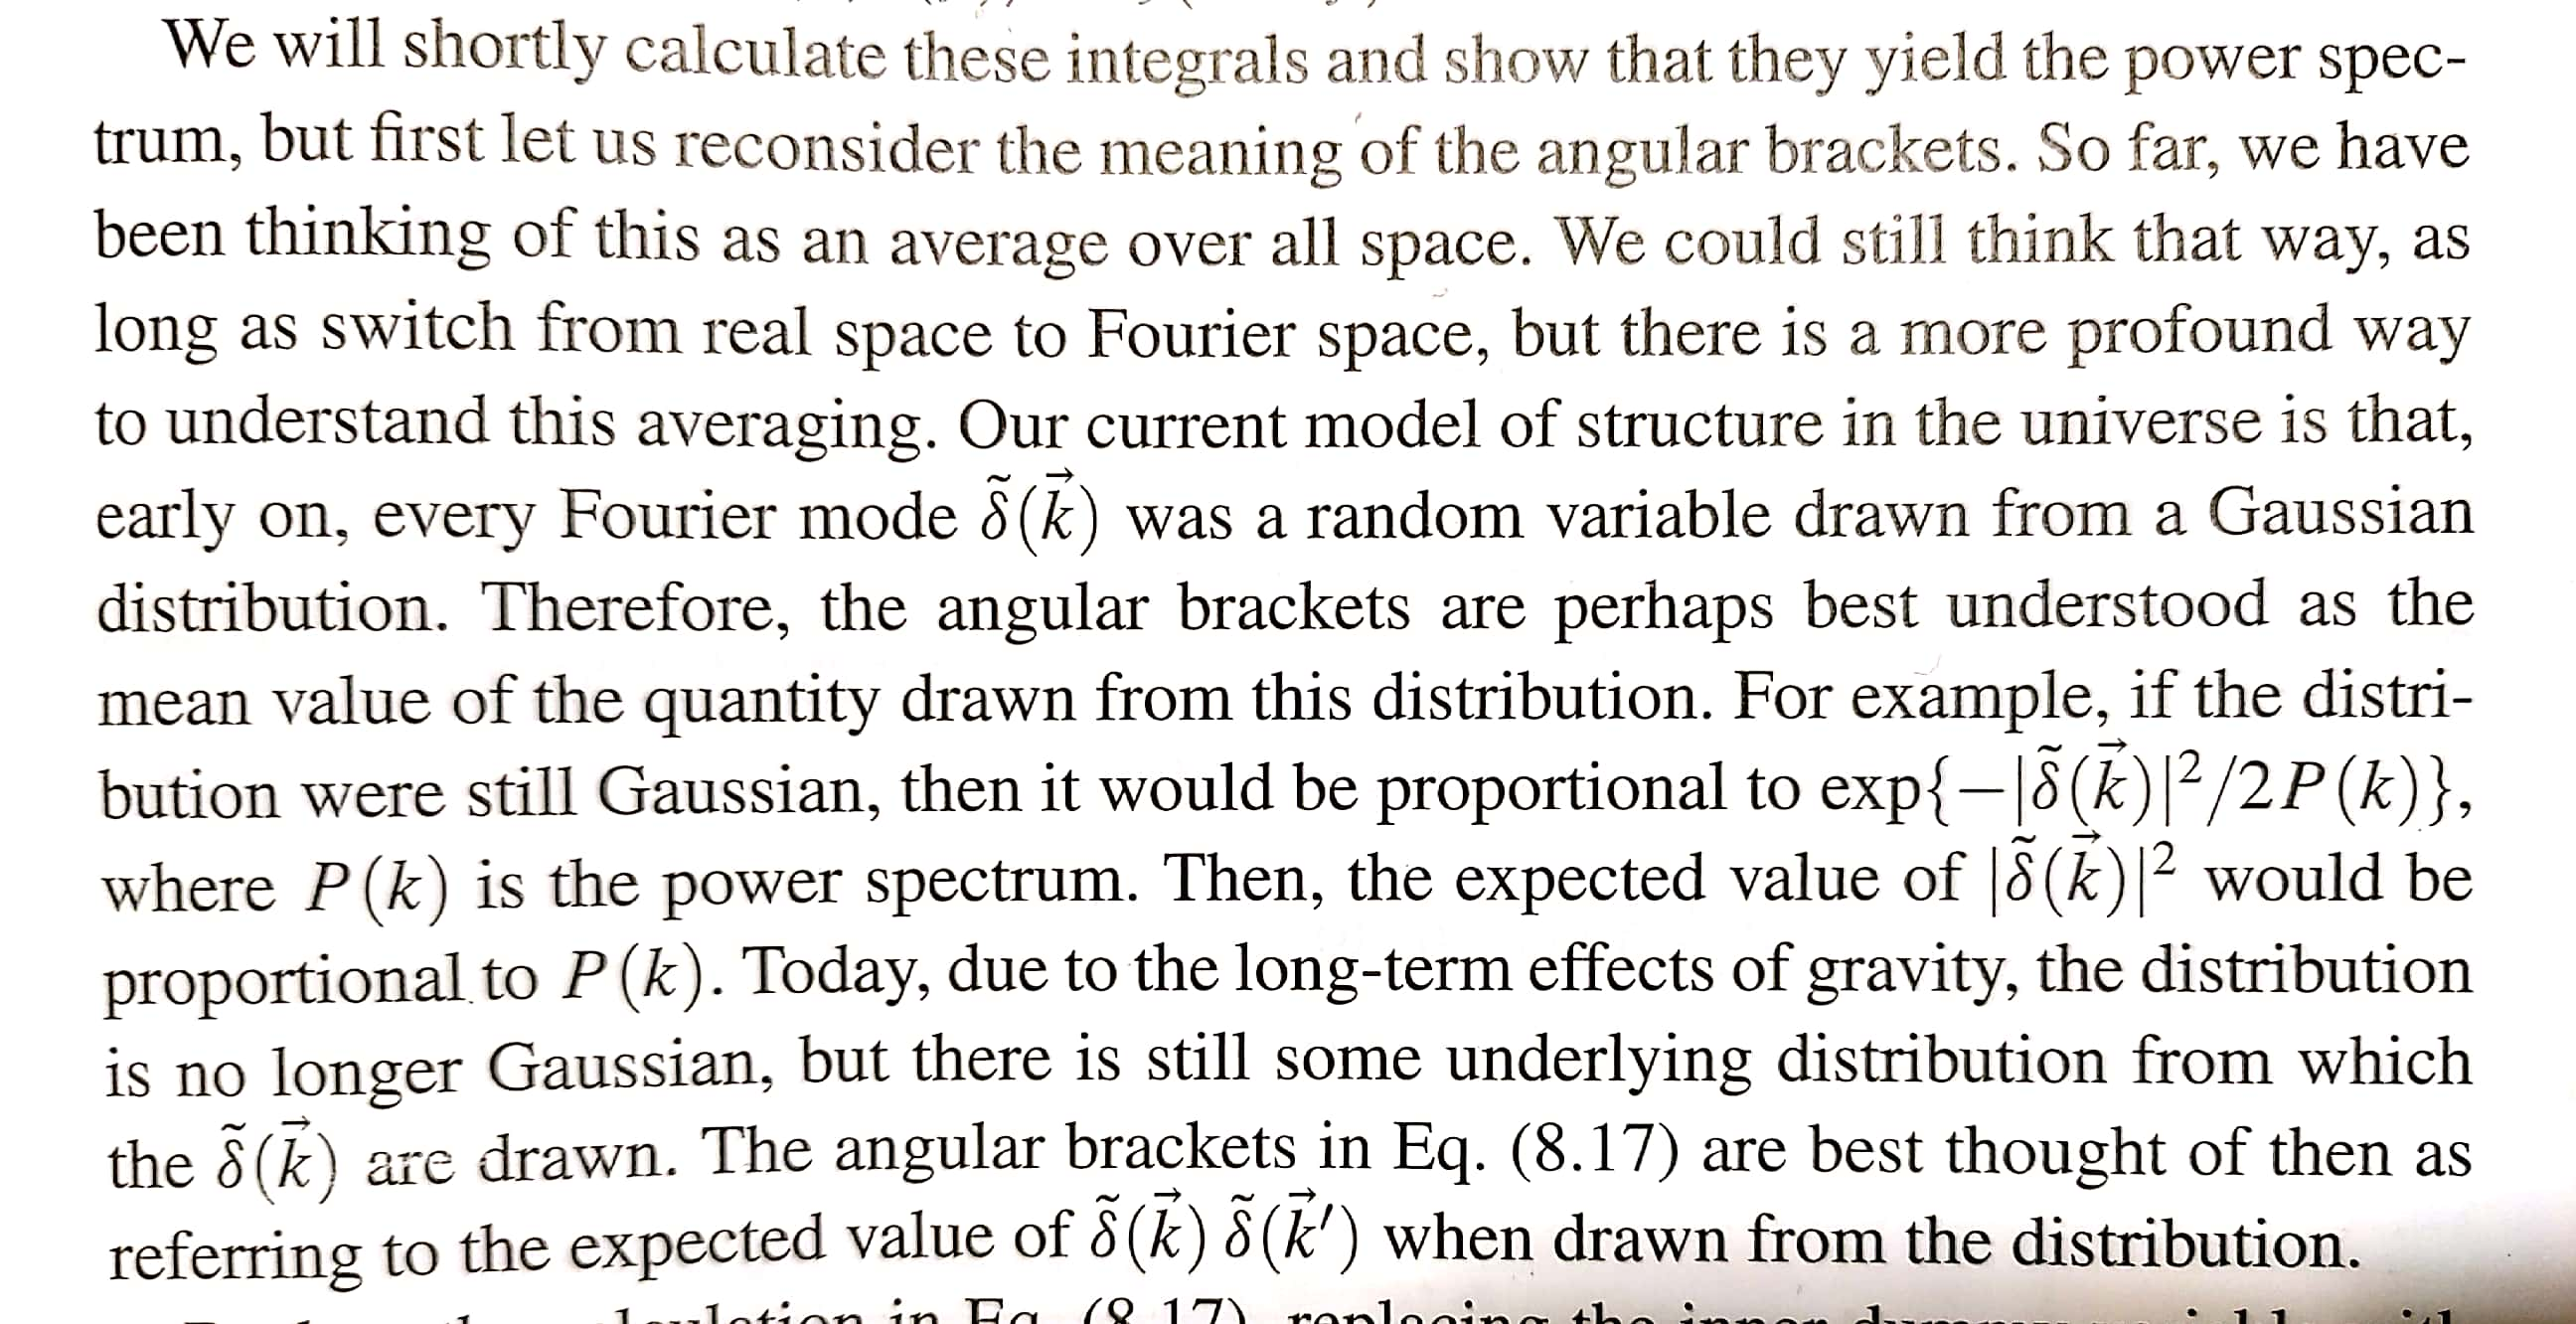
\includegraphics[width=0.9\linewidth]{../images/brackets}
	\caption{}
	\label{fig:brackets}
\end{figure}



\subsection{power spectrum}
Now, we define the correlation function as
\beq
\beqal
\langle \delta(\kappa) \delta(\kappa) \rangle &=  \int dx  \int dy e^{-\kappa \cdot x} e^{-\kappa' \cdot y} \langle  \delta(x) \delta(y) \rangle
\\
&= \int dx \int dy e^{-\kappa \cdot x} e^{-\kappa' \cdot y}  \xi(x - y)
\\
&= \int dx \int dy e^{-(\kappa + \kappa') \cdot x} e^{\kappa' \cdot (x-y)}  \xi(x - y)
\\
&= \int dx e^{(\kappa + \kappa') \cdot x} \int dx_d  e^{\kappa' \cdot (x_d)}  \xi(x_d)
\\
&= 2\pi \delta(\kappa + \kappa') P(k') \label{eq:correlation_function}
\eeqal
\eeq

where, in the fourth equality  $ (x-y) $ was replaced by $ x_d $. Minus sign coming from $ -dx_d $ was cancelled by the change of variable $ x \rightarrow -x $. $ P(k) $ is called as the power spectrum. In this case it's a 3d power spectrum.

\end{document}

